\section{Trusted Path to Remote Enclave} 
\label{sec:trustedPathAppendix}


%\begin{figure*}[t]
% \centering
%  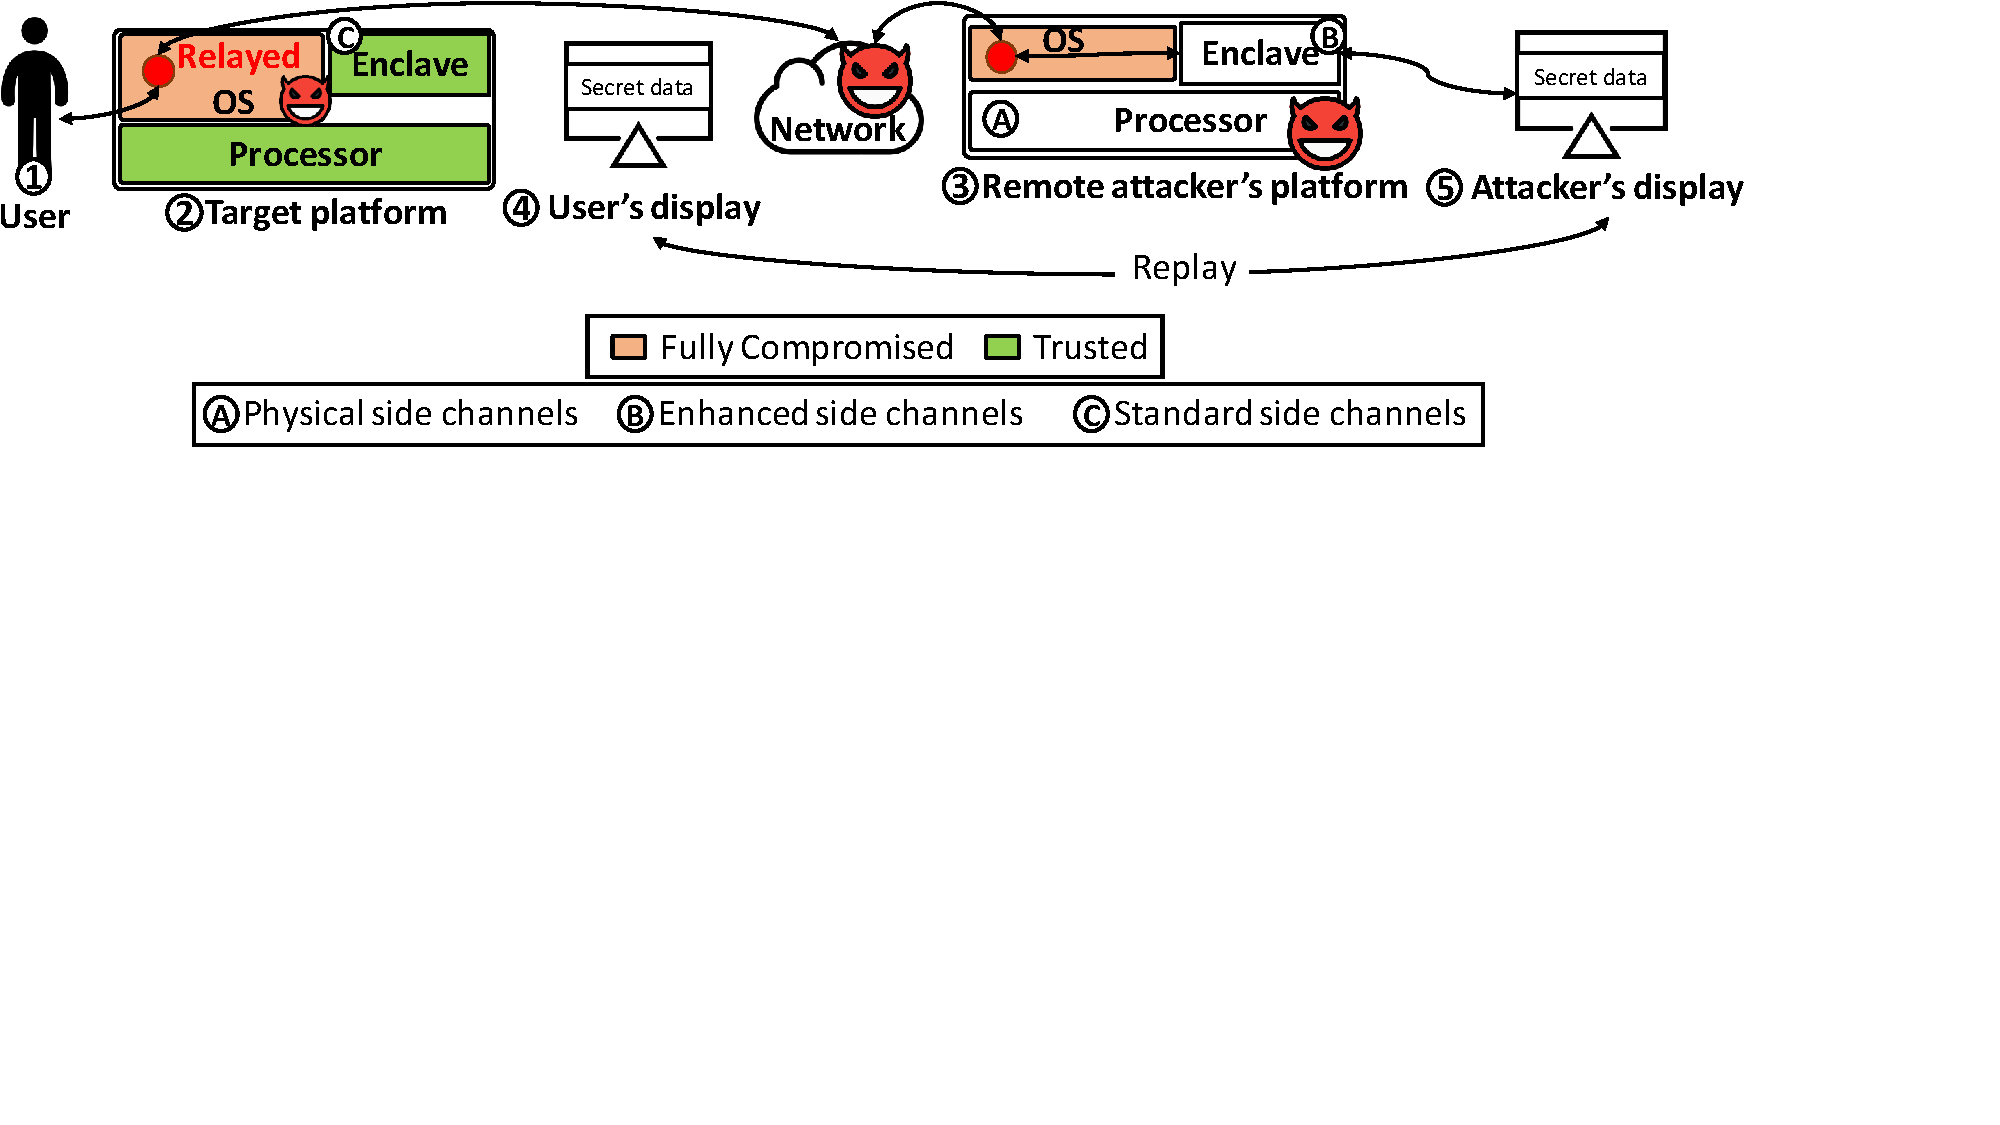
\includegraphics[trim={0cm 11cm 4cm 0},clip,width=0.7\linewidth]{trustedPathRelay.pdf}
% \caption{The figure illustrates relay attack on trusted path where the attacker sees all the sensitive input from the user on his display that is connected to the attacker's enclave. The user sees a replay of the attacker's display.}
%	%\figsaver
% \label{fig:trustedPathRelay}
%\end{figure*}

%\subsection{Relay Attack on Trusted Path}
%\label{sec:trustedPathAppendix:relay}
%
%Figure~\ref{fig:trustedPathRelay} relay attack on the trusted path. Assume the user has a trusted path between her Io devices and the SGX enclave. The enclave implements IO drivers (e.g., keyboard, mouse, display, etc.) to provide a trusted path. Here the attacker captures all the input from the user as they appear on the attacker display, for example, credit card number, selection of a candidate in e-voting portal, etc. Then the attacker replays back his display back to the user. The user cannot distinguish if the display is coming from her local enclave or she is observing a remote desktop session from the attacker. Thus, the relay attack breaks the security property of the trusted path.


\begin{figure}[t]
 \centering
  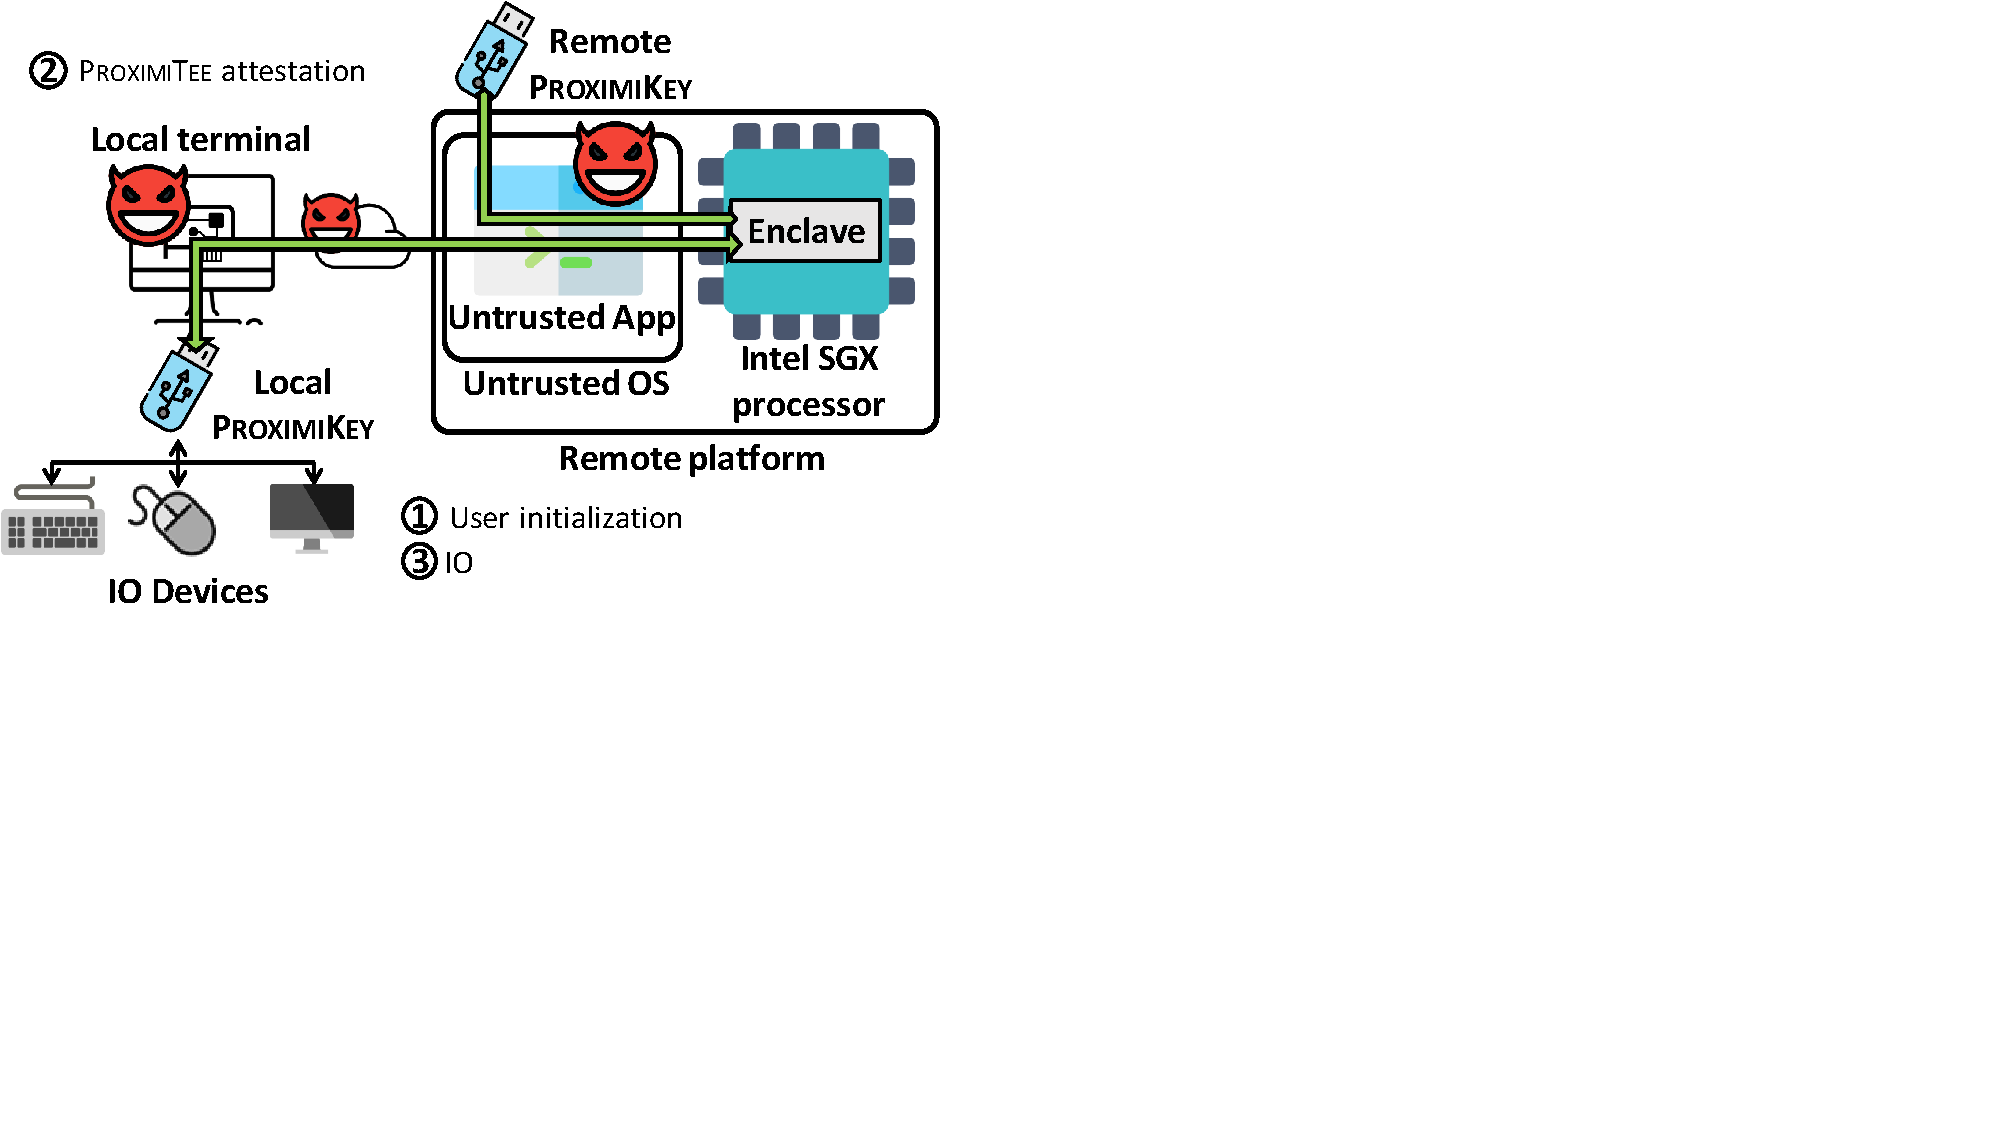
\includegraphics[trim={0cm 8.6cm 18cm 0},clip,width=0.8\linewidth]{RemoteEnclaveTrustedPath.pdf}
 \caption{Trusted path to remote enclave. This setup uses two embedded devices. The local \device is connected to the local platform and the remote \device is connected with the remote platform.}
	\figsaver
 \label{fig:systemRemoteHost}
\end{figure}

%\subsection{Trusted Path to Remote Enclave}
%\label{sec:trustedPathAppendix:remoteEnclave}

In this appendix we describe how a \emph{local} trusted path, described in Section~\ref{sec:secureInput}, can be extended to an enclave that resides on a \emph{remote} platform, as shown in Figure~\ref{fig:systemRemoteHost}. Both the local and the remote platform have a \device device attached to them. The I/O devices are attached to the local \device. Trusted path creation proceeds as follows:

\begin{mylist}
	\item[\one] The user initiates the trusted path by selecting an enclave as explained above.
	\item[\two] The local \device acts as the remote verifier in remote attestation using using one of our attestation mechanisms. As the end result of the attestation process, the local \device has established a secure channel to the correct enclave via the remote \device.
	\item[\three] The user can securely communicate with the enclave.
\end{mylist}




